% Options for packages loaded elsewhere
% Options for packages loaded elsewhere
\PassOptionsToPackage{unicode}{hyperref}
\PassOptionsToPackage{hyphens}{url}
\PassOptionsToPackage{dvipsnames,svgnames,x11names}{xcolor}
%
\documentclass[
  11pt,
  letterpaper,
  DIV=11,
  numbers=noendperiod]{scrartcl}
\usepackage{xcolor}
\usepackage[top=30mm,left=25mm,right=25mm,bottom=30mm]{geometry}
\usepackage{amsmath,amssymb}
\setcounter{secnumdepth}{2}
\usepackage{iftex}
\ifPDFTeX
  \usepackage[T1]{fontenc}
  \usepackage[utf8]{inputenc}
  \usepackage{textcomp} % provide euro and other symbols
\else % if luatex or xetex
  \usepackage{unicode-math} % this also loads fontspec
  \defaultfontfeatures{Scale=MatchLowercase}
  \defaultfontfeatures[\rmfamily]{Ligatures=TeX,Scale=1}
\fi
\usepackage{lmodern}
\ifPDFTeX\else
  % xetex/luatex font selection
\fi
% Use upquote if available, for straight quotes in verbatim environments
\IfFileExists{upquote.sty}{\usepackage{upquote}}{}
\IfFileExists{microtype.sty}{% use microtype if available
  \usepackage[]{microtype}
  \UseMicrotypeSet[protrusion]{basicmath} % disable protrusion for tt fonts
}{}
\usepackage{setspace}
\makeatletter
\@ifundefined{KOMAClassName}{% if non-KOMA class
  \IfFileExists{parskip.sty}{%
    \usepackage{parskip}
  }{% else
    \setlength{\parindent}{0pt}
    \setlength{\parskip}{6pt plus 2pt minus 1pt}}
}{% if KOMA class
  \KOMAoptions{parskip=half}}
\makeatother
% Make \paragraph and \subparagraph free-standing
\makeatletter
\ifx\paragraph\undefined\else
  \let\oldparagraph\paragraph
  \renewcommand{\paragraph}{
    \@ifstar
      \xxxParagraphStar
      \xxxParagraphNoStar
  }
  \newcommand{\xxxParagraphStar}[1]{\oldparagraph*{#1}\mbox{}}
  \newcommand{\xxxParagraphNoStar}[1]{\oldparagraph{#1}\mbox{}}
\fi
\ifx\subparagraph\undefined\else
  \let\oldsubparagraph\subparagraph
  \renewcommand{\subparagraph}{
    \@ifstar
      \xxxSubParagraphStar
      \xxxSubParagraphNoStar
  }
  \newcommand{\xxxSubParagraphStar}[1]{\oldsubparagraph*{#1}\mbox{}}
  \newcommand{\xxxSubParagraphNoStar}[1]{\oldsubparagraph{#1}\mbox{}}
\fi
\makeatother


\usepackage{longtable,booktabs,array}
\usepackage{calc} % for calculating minipage widths
% Correct order of tables after \paragraph or \subparagraph
\usepackage{etoolbox}
\makeatletter
\patchcmd\longtable{\par}{\if@noskipsec\mbox{}\fi\par}{}{}
\makeatother
% Allow footnotes in longtable head/foot
\IfFileExists{footnotehyper.sty}{\usepackage{footnotehyper}}{\usepackage{footnote}}
\makesavenoteenv{longtable}
\usepackage{graphicx}
\makeatletter
\newsavebox\pandoc@box
\newcommand*\pandocbounded[1]{% scales image to fit in text height/width
  \sbox\pandoc@box{#1}%
  \Gscale@div\@tempa{\textheight}{\dimexpr\ht\pandoc@box+\dp\pandoc@box\relax}%
  \Gscale@div\@tempb{\linewidth}{\wd\pandoc@box}%
  \ifdim\@tempb\p@<\@tempa\p@\let\@tempa\@tempb\fi% select the smaller of both
  \ifdim\@tempa\p@<\p@\scalebox{\@tempa}{\usebox\pandoc@box}%
  \else\usebox{\pandoc@box}%
  \fi%
}
% Set default figure placement to htbp
\def\fps@figure{htbp}
\makeatother





\setlength{\emergencystretch}{3em} % prevent overfull lines

\providecommand{\tightlist}{%
  \setlength{\itemsep}{0pt}\setlength{\parskip}{0pt}}



 


\usepackage{booktabs}
\usepackage{longtable}
\usepackage{array}
\usepackage{multirow}
\usepackage{wrapfig}
\usepackage{float}
\usepackage{colortbl}
\usepackage{pdflscape}
\usepackage{tabu}
\usepackage{threeparttable}
\usepackage{threeparttablex}
\usepackage[normalem]{ulem}
\usepackage{makecell}
\usepackage{xcolor}
\usepackage{fvextra}
\DefineVerbatimEnvironment{Highlighting}{Verbatim}{breaklines,commandchars=\\\{\}}
\usepackage{booktabs}
\usepackage{longtable}
\usepackage{array}
\usepackage{caption}
\usepackage{float}
\setlength{\emergencystretch}{3em}
\KOMAoption{captions}{tableheading}
\makeatletter
\@ifpackageloaded{caption}{}{\usepackage{caption}}
\AtBeginDocument{%
\ifdefined\contentsname
  \renewcommand*\contentsname{Table of contents}
\else
  \newcommand\contentsname{Table of contents}
\fi
\ifdefined\listfigurename
  \renewcommand*\listfigurename{List of Figures}
\else
  \newcommand\listfigurename{List of Figures}
\fi
\ifdefined\listtablename
  \renewcommand*\listtablename{List of Tables}
\else
  \newcommand\listtablename{List of Tables}
\fi
\ifdefined\figurename
  \renewcommand*\figurename{Figure}
\else
  \newcommand\figurename{Figure}
\fi
\ifdefined\tablename
  \renewcommand*\tablename{Table}
\else
  \newcommand\tablename{Table}
\fi
}
\@ifpackageloaded{float}{}{\usepackage{float}}
\floatstyle{ruled}
\@ifundefined{c@chapter}{\newfloat{codelisting}{h}{lop}}{\newfloat{codelisting}{h}{lop}[chapter]}
\floatname{codelisting}{Listing}
\newcommand*\listoflistings{\listof{codelisting}{List of Listings}}
\makeatother
\makeatletter
\makeatother
\makeatletter
\@ifpackageloaded{caption}{}{\usepackage{caption}}
\@ifpackageloaded{subcaption}{}{\usepackage{subcaption}}
\makeatother
\usepackage{bookmark}
\IfFileExists{xurl.sty}{\usepackage{xurl}}{} % add URL line breaks if available
\urlstyle{same}
\hypersetup{
  pdftitle={Taller 1: Análisis de Demanda y Endogeneidad},
  pdfauthor={Juan Diego Moreno Sánchez},
  colorlinks=true,
  linkcolor={blue},
  filecolor={Maroon},
  citecolor={Blue},
  urlcolor={Blue},
  pdfcreator={LaTeX via pandoc}}


\title{Taller 1: Análisis de Demanda y Endogeneidad}
\usepackage{etoolbox}
\makeatletter
\providecommand{\subtitle}[1]{% add subtitle to \maketitle
  \apptocmd{\@title}{\par {\large #1 \par}}{}{}
}
\makeatother
\subtitle{Tópicos en Econometría}
\author{Juan Diego Moreno Sánchez}
\date{2026-03-16}
\begin{document}
\maketitle


\setstretch{1.15}
\section{EJERCICIO 1 -- Pronosticando la Brecha de Género en el Mercado
Laboral
Colombiano}\label{ejercicio-1-pronosticando-la-brecha-de-guxe9nero-en-el-mercado-laboral-colombiano}

Usted(es) han sido contratados por una ONG para participar como
consultores cuantitativos en un proyecto sobre brechas de género en el
mercado laboral. Dados sus conocimientos en Series de Tiempo, el líder
del proyecto les asigna la tarea de elaborar un análisis estadístico de
series de tiempo de la tasa de desempleo para hombres y la tasa de
desempleo para mujeres en Colombia, con el fin de pronosticar y después
calcular la brecha de género. Para esto ustedes deben construir una base
de datos para el periodo mensual de 2007M1 a 2025M12. Para estructurar
su análisis, el líder les indica los siguientes pasos a seguir:

\subsection{a) Presente una gráfica de ambas series de tiempo. Describa
el comportamiento de la tendencia a lo largo de la serie y de la
estacionalidad. Puede acompañar esto con una gráfica estacional
(seasonal graph) de cada
serie.}\label{a-presente-una-gruxe1fica-de-ambas-series-de-tiempo.-describa-el-comportamiento-de-la-tendencia-a-lo-largo-de-la-serie-y-de-la-estacionalidad.-puede-acompauxf1ar-esto-con-una-gruxe1fica-estacional-seasonal-graph-de-cada-serie.}

En la siguiente grafica podremos observar el comportamiento de ambas
series a lo largo del tiempo, así como su estacionalidad.

A primera vista podemos ver que el desempleo de mujeres es más alto que
el de los hombre, incluso la serie de las mujeres tiene un componente
estacional multiplicativo, mientras que la serie de los hombres tiene un
componente estacional aditivo. Además, ambas series presentan una
tendencia creciente a lo largo del tiempo, aunque la tasa de desempleo
de mujeres parece tener una tendencia más pronunciada que la de los
hombres. En cuanto a la estacionalidad, se observa que ambos series
presentan picos en ciertos meses del año, lo que sugiere la presencia de
estacionalidad en ambas series. Sin embargo, la estacionalidad en la
serie de mujeres parece ser más fuerte que en la serie de hombres.

\begin{figure}

\centering{

\pandocbounded{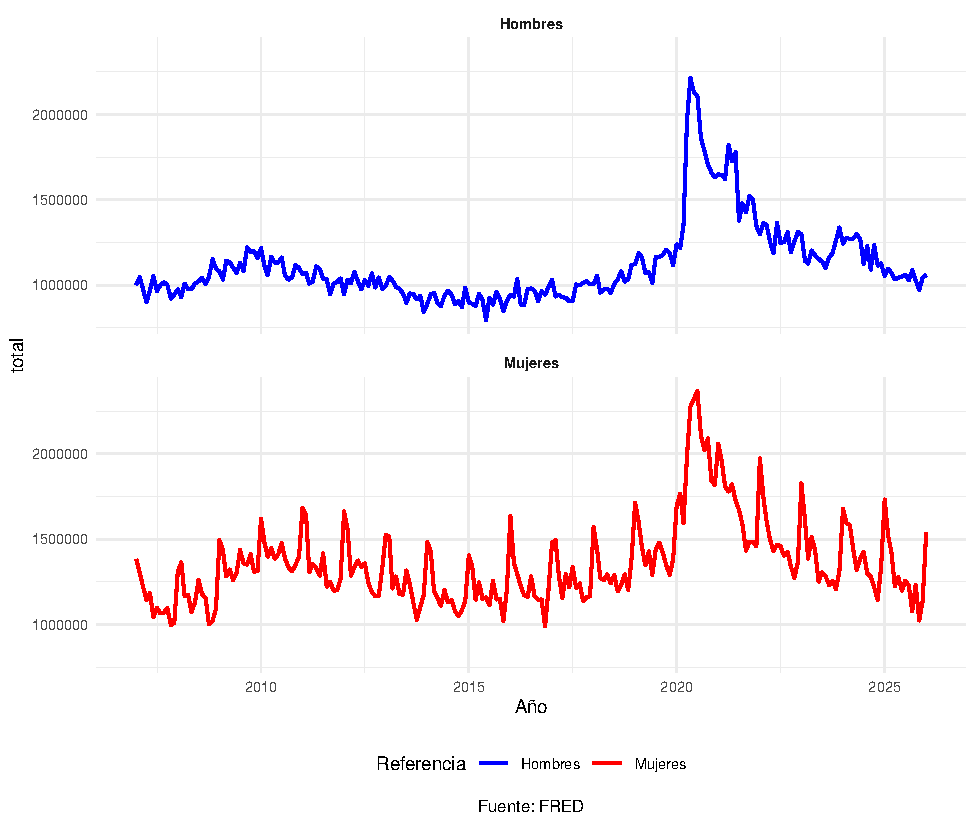
\includegraphics[keepaspectratio]{1TallerParcial_files/figure-pdf/fig-desempleo-1.pdf}}

}

\caption{\label{fig-desempleo}Desempleo en Colombia por Sexo
(2007-2025)}

\end{figure}%

\subsection{b) Construya una tabla para cada serie donde presente por
cada año (2007 a 2025) la media, la mediana, la desviación estándar, el
mínimo y el máximo. Redacte dos párrafos en los que utilice estos
estadísticos para comparar las
series.}\label{b-construya-una-tabla-para-cada-serie-donde-presente-por-cada-auxf1o-2007-a-2025-la-media-la-mediana-la-desviaciuxf3n-estuxe1ndar-el-muxednimo-y-el-muxe1ximo.-redacte-dos-puxe1rrafos-en-los-que-utilice-estos-estaduxedsticos-para-comparar-las-series.}

\begingroup\fontsize{10}{12}\selectfont

\begin{longtable}[t]{ccccc}
\caption{\label{tab:unnamed-chunk-2}Análisis de Brechas de Género en el Desempleo (2007-2025)}\\
\toprule
\multicolumn{1}{c}{ } & \multicolumn{4}{c}{Métricas de Desigualdad (Mujeres vs. Hombres)} \\
\cmidrule(l{3pt}r{3pt}){2-5}
Año & Dif. total & Razón (W/M) & Dif. SD & Dif. Máximos\\
\midrule
\cellcolor{gray!10}{2007} & \cellcolor{gray!10}{151440.9} & \cellcolor{gray!10}{1.15} & \cellcolor{gray!10}{71932.36} & \cellcolor{gray!10}{329864.0}\\
2008 & 139191.8 & 1.14 & 50420.94 & 212051.0\\
\cellcolor{gray!10}{2009} & \cellcolor{gray!10}{226437.8} & \cellcolor{gray!10}{1.20} & \cellcolor{gray!10}{14356.15} & \cellcolor{gray!10}{272171.0}\\
2010 & 304518.8 & 1.27 & 26152.70 & 402664.0\\
\cellcolor{gray!10}{2011} & \cellcolor{gray!10}{307793.1} & \cellcolor{gray!10}{1.30} & \cellcolor{gray!10}{117131.26} & \cellcolor{gray!10}{571597.0}\\
\addlinespace
2012 & 319285.0 & 1.31 & 109983.63 & 583998.0\\
\cellcolor{gray!10}{2013} & \cellcolor{gray!10}{281617.5} & \cellcolor{gray!10}{1.29} & \cellcolor{gray!10}{95782.45} & \cellcolor{gray!10}{476813.0}\\
2014 & 260664.0 & 1.28 & 97083.61 & 498598.3\\
\cellcolor{gray!10}{2015} & \cellcolor{gray!10}{296320.4} & \cellcolor{gray!10}{1.33} & \cellcolor{gray!10}{58441.97} & \cellcolor{gray!10}{442042.8}\\
2016 & 281005.4 & 1.30 & 112940.48 & 600090.0\\
\addlinespace
\cellcolor{gray!10}{2017} & \cellcolor{gray!10}{296393.1} & \cellcolor{gray!10}{1.31} & \cellcolor{gray!10}{71856.76} & \cellcolor{gray!10}{460357.0}\\
2018 & 287598.5 & 1.28 & 58611.62 & 450431.0\\
\cellcolor{gray!10}{2019} & \cellcolor{gray!10}{295008.8} & \cellcolor{gray!10}{1.26} & \cellcolor{gray!10}{64435.40} & \cellcolor{gray!10}{505925.0}\\
2020 & 251012.6 & 1.14 & -86888.21 & 156362.0\\
\cellcolor{gray!10}{2021} & \cellcolor{gray!10}{114641.7} & \cellcolor{gray!10}{1.07} & \cellcolor{gray!10}{48483.40} & \cellcolor{gray!10}{238601.0}\\
\addlinespace
2022 & 215872.0 & 1.17 & 132301.24 & 607855.0\\
\cellcolor{gray!10}{2023} & \cellcolor{gray!10}{194290.1} & \cellcolor{gray!10}{1.16} & \cellcolor{gray!10}{112228.33} & \cellcolor{gray!10}{488385.0}\\
2024 & 178753.4 & 1.15 & 84268.62 & 379479.0\\
\cellcolor{gray!10}{2025} & \cellcolor{gray!10}{230349.4} & \cellcolor{gray!10}{1.22} & \cellcolor{gray!10}{164436.87} & \cellcolor{gray!10}{634776.0}\\
2026 & 476878.0 & 1.45 & NA & 476878.0\\
\bottomrule
\multicolumn{5}{l}{\rule{0pt}{1em}Fuente: Elaboración propia con datos de FRED (Federal Reserve Economic Data).}\\
\end{longtable}
\endgroup{}

Para esta tabla tome la desición por orden e intepretabilidad de que los
estaditicos no sean por separado para cada serie, sino que se muestren
las diferencias entre ambas series. Esto con el fin de facilitar la
comparación entre las dos series. En esta tabla se pueden observar
varias métricas que permiten comparar la tasa de desempleo entre hombres
y mujeres a lo largo del tiempo. La columna ``Dif. total'' muestra la
diferencia en la media de desempleo entre mujeres y hombres para cada
año, evidenciando que en todos los años las mujeres tienen una tasa de
desempleo más alta que los hombres. La columna ``Razón (W/M)'' indica
cuántas veces es mayor la tasa de desempleo de las mujeres en
comparación con la de los hombres, mostrando una tendencia creciente a
lo largo del tiempo, lo que sugiere un aumento en la brecha de género en
el desempleo. La columna ``Dif. SD'' muestra la diferencia en la
desviación estándar entre las dos series, indicando que la volatilidad
del desempleo para las mujeres es generalmente mayor que para los
hombres, lo que podría reflejar una mayor inestabilidad en el mercado
laboral para las mujeres. Finalmente, la columna ``Dif. Máximos''
muestra la diferencia en los valores máximos de desempleo entre mujeres
y hombres, evidenciando que en los años de crisis económica, como 2020,
la brecha en los picos de desempleo se amplió significativamente, lo que
podría estar relacionado con el impacto desproporcionado de la pandemia
en ciertos sectores donde las mujeres tienen una mayor representación.

\subsection{c) Utilizando la metodología de Box-Jenkins, determine el
mejor modelo SARIMA que represente el Proceso Generador de Datos de cada
serie. Esto debe estar acompañado de las pruebas necesarias y la
justificación de su
elección.}\label{c-utilizando-la-metodologuxeda-de-box-jenkins-determine-el-mejor-modelo-sarima-que-represente-el-proceso-generador-de-datos-de-cada-serie.-esto-debe-estar-acompauxf1ado-de-las-pruebas-necesarias-y-la-justificaciuxf3n-de-su-elecciuxf3n.}

\subsection{d) Realice un pronóstico de la tasa de desempleo de hombres
y de la tasa de desempleo de mujeres para los doce meses del año 2026.
Presente un gráfico con ambas series.
Comente.}\label{d-realice-un-pronuxf3stico-de-la-tasa-de-desempleo-de-hombres-y-de-la-tasa-de-desempleo-de-mujeres-para-los-doce-meses-del-auxf1o-2026.-presente-un-gruxe1fico-con-ambas-series.-comente.}

\subsubsection{1. Serie de desempleo de
mujeres}\label{serie-de-desempleo-de-mujeres}

\begin{enumerate}
\def\labelenumi{\arabic{enumi}.}
\tightlist
\item
  Primero haremos toda la metodología de Box-Jenkins para la serie de
  desempleo de mujeres, y luego para la serie de desempleo de hombres.
  Para cada serie, se realizará el análisis de estacionariedad,
  identificación del modelo SARIMA, estimación de parámetros,
  diagnóstico del modelo y finalmente el pronóstico para el año 2026.
\end{enumerate}

La visualización de las serie de desempleo de mujeres muestra una
tendencia creciente y una estacionalidad clara, lo que sugiere que la
serie no es estacionaria. Para confirmar esto, se realizará la prueba de
Dickey-Fuller aumentada (ADF) para verificar la presencia de raíces
unitarias. Si la serie no es estacionaria, se aplicará una
diferenciación para eliminar la tendencia y/o estacionalidad.

\begin{verbatim}

    Augmented Dickey-Fuller Test

data:  unemployment_data$unemployment_w
Dickey-Fuller = -3.0045, Lag order = 6, p-value = 0.1539
alternative hypothesis: stationary
\end{verbatim}

La prueba ADF nos dice que la serie de desempleo de mujeres no es
estacionaria, ya que el valor p es mayor que 0.05. Por lo tanto, se
aplicará una diferenciación para eliminar la tendencia y/o
estacionalidad.

\begin{verbatim}

    Augmented Dickey-Fuller Test

data:  unemployment_w_diff
Dickey-Fuller = -7.0311, Lag order = 6, p-value = 0.01
alternative hypothesis: stationary
\end{verbatim}

La serie diferenciada del desempleo en mujeres ahora es estacionaria,
gracias a que la prueba ADF muestra un valor p de 0.01, lo que indica
que podemos proceder a la identificación del proceso SARIMA para esta
serie. Se analizarán los gráficos de autocorrelación (ACF) y
autocorrelación parcial (PACF) para determinar los posibles valores de
los parámetros p, d, q, P, D, Q y m.

\pandocbounded{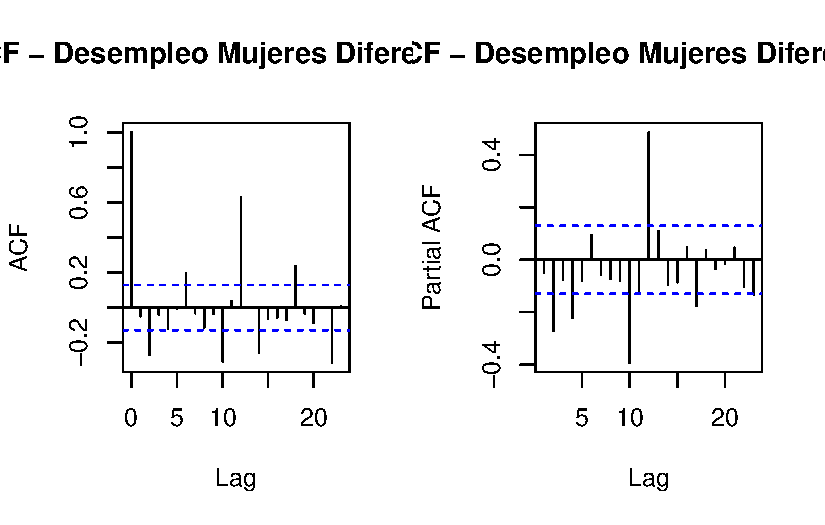
\includegraphics[keepaspectratio]{1TallerParcial_files/figure-pdf/unnamed-chunk-5-1.pdf}}

Podemos observar como el resago 12 muestra una autocorrelación
significativa, lo que sugiere la presencia de estacionalidad anual.
Además, los primeros rezagos también muestran autocorrelación, lo que
indica que podríamos considerar un modelo SARIMA con componentes tanto
no estacionales como estacionales. Basándonos en estos gráficos, se
podrían probar varios modelos SARIMA, como SARIMA(1,1,1)(1,1,1){[}12{]},
SARIMA(0,1,1)(0,1,1){[}12{]}, entre otros. La selección del mejor modelo
se realizará utilizando criterios de información como AIC o BIC.

\newpage

\begingroup\fontsize{10}{12}\selectfont

\begin{longtable}[t]{ccc}
\caption{\label{tab:unnamed-chunk-6}Comparación de Modelos SARIMA para Desempleo de Mujeres}\\
\toprule
Modelo & AIC & BIC\\
\midrule
\cellcolor{gray!10}{SARIMA(1,1,1)(1,1,1)[12]} & \cellcolor{gray!10}{5556.594} & \cellcolor{gray!10}{5573.471}\\
SARIMA(0,1,1)(0,1,1)[12] & 5554.984 & 5565.110\\
\cellcolor{gray!10}{Auto ARIMA} & \cellcolor{gray!10}{6053.219} & \cellcolor{gray!10}{6066.936}\\
\bottomrule
\multicolumn{3}{l}{\rule{0pt}{1em}Fuente: Elaboración propia con datos de FRED (Federal Reserve Economic Data).}\\
\end{longtable}
\endgroup{}

De nuevo podemos ver que el auto.arima es el modelo que peor resultado
da, mientras que el modelo SARIMA(0,1,1)(0,1,1){[}12{]} es el que mejor
resultado da, con el menor AIC y BIC. Por lo tanto, se seleccionará el
modelo SARIMA(0,1,1)(0,1,1){[}12{]} para la serie de desempleo de
mujeres. Se realizará un diagnóstico del modelo para verificar que los
residuos sean ruido blanco y luego se procederá a realizar el pronóstico
para el año 2026.

\pandocbounded{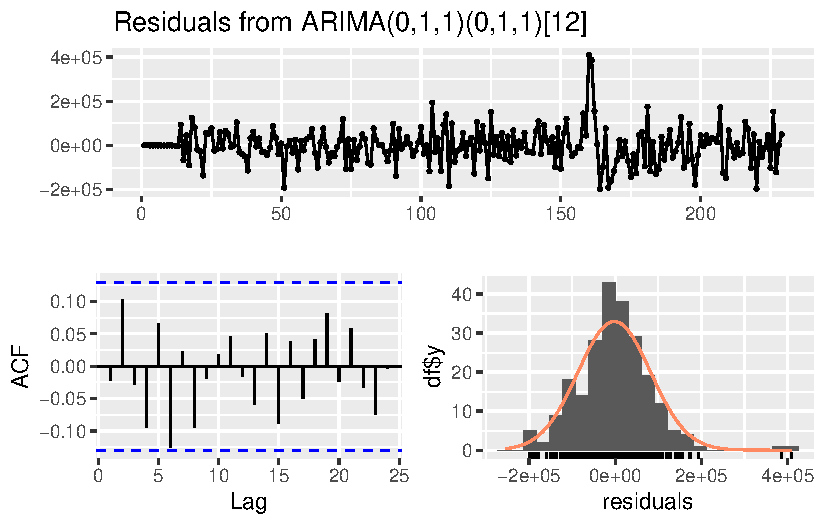
\includegraphics[keepaspectratio]{1TallerParcial_files/figure-pdf/unnamed-chunk-7-1.pdf}}

\begin{verbatim}

    Ljung-Box test

data:  Residuals from ARIMA(0,1,1)(0,1,1)[12]
Q* = 12.048, df = 8, p-value = 0.1491

Model df: 2.   Total lags used: 10
\end{verbatim}

\begin{verbatim}

    Box-Ljung test

data:  residuals(model_w_2)
X-squared = 19.266, df = 20, p-value = 0.5046
\end{verbatim}

Podemos ver que el modelo SARIMA(0,1,1)(0,1,1){[}12{]} para la serie de
desempleo de mujeres tiene residuos que parecen ser ruido blanco, ya que
no muestran patrones significativos en el gráfico de residuos ni en el
gráfico de ACF de los residuos. Además, la prueba de Ljung-Box no es
significativa, lo que indica que no hay autocorrelación en los residuos.
Por lo tanto, se puede concluir que el modelo es adecuado para
representar la serie de desempleo de mujeres. A continuación, se
realizará el pronóstico para los doce meses del año 2026 utilizando este
modelo.

La predicción para el año 2026 se realizará utilizando la función
\texttt{forecast} del paquete \texttt{forecast}, que nos permitirá
obtener los valores pronosticados para cada mes de 2026, así como los
intervalos de confianza asociados a estos pronósticos. Luego, se
graficarán los resultados para visualizar tanto la serie histórica como
los pronósticos para el año 2026.

\pandocbounded{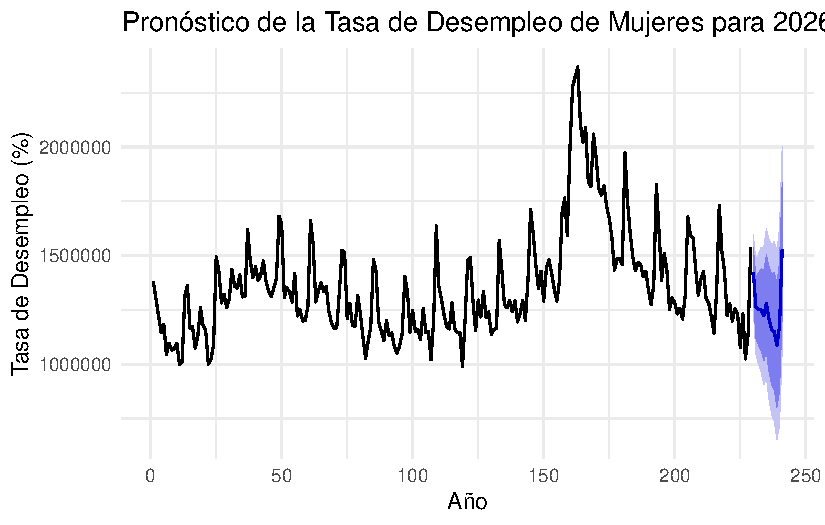
\includegraphics[keepaspectratio]{1TallerParcial_files/figure-pdf/unnamed-chunk-8-1.pdf}}

Podemos observar que el modelo predice un ciclo de caida del desempleo
en mujeres para el año 2026.

\subsubsection{2. Serie de desempleo de
hombres}\label{serie-de-desempleo-de-hombres}

\begin{enumerate}
\def\labelenumi{\arabic{enumi}.}
\setcounter{enumi}{1}
\tightlist
\item
  Para la serie de desempleo de hombres, se realizará el mismo proceso
  de análisis de estacionariedad, identificación del modelo SARIMA,
  estimación de parámetros, diagnóstico del modelo y pronóstico para el
  año 2026. Se espera encontrar un modelo SARIMA diferente al de la
  serie de mujeres, dado que las características de ambas series son
  distintas en términos de tendencia y estacionalidad.
\end{enumerate}

Realizaremos la prueba de Dickey-Fuller aumentada para la serie de
desempleo de hombres para verificar su estacionariedad, y en caso de no
ser estacionaria, se aplicará una diferenciación similar a la realizada
para la serie de mujeres. Luego, se analizarán los gráficos de ACF y
PACF para identificar los posibles modelos SARIMA y se seleccionará el
mejor modelo utilizando criterios de información como AIC o BIC.
Finalmente, se realizará el diagnóstico del modelo seleccionado y se
procederá a realizar el pronóstico para el año 2026.

\begin{verbatim}

    Augmented Dickey-Fuller Test

data:  m_ts
Dickey-Fuller = -2.175, Lag order = 6, p-value = 0.5024
alternative hypothesis: stationary
\end{verbatim}

Podemos ver que la serie de desempleo de hombres también no es
estacionaria, ya que el valor p es mayor que 0.10. Por lo tanto, se
aplicará una diferenciación para eliminar la tendencia y/o
estacionalidad.

\begin{verbatim}

    Augmented Dickey-Fuller Test

data:  unemployment_m_diff
Dickey-Fuller = -6.619, Lag order = 6, p-value = 0.01
alternative hypothesis: stationary
\end{verbatim}

Ahora la serie diferenciada del desempleo en hombres es estacionaria,
con un valor p de 0.01. Por lo tanto, se puede proceder a la
identificación del proceso SARIMA para esta serie, analizando los
gráficos de ACF y PACF para determinar los posibles valores de los
parámetros p, d, q, P, D, Q y m. Se probarán varios modelos SARIMA y se
seleccionará el mejor utilizando criterios de información como AIC o
BIC.

\pandocbounded{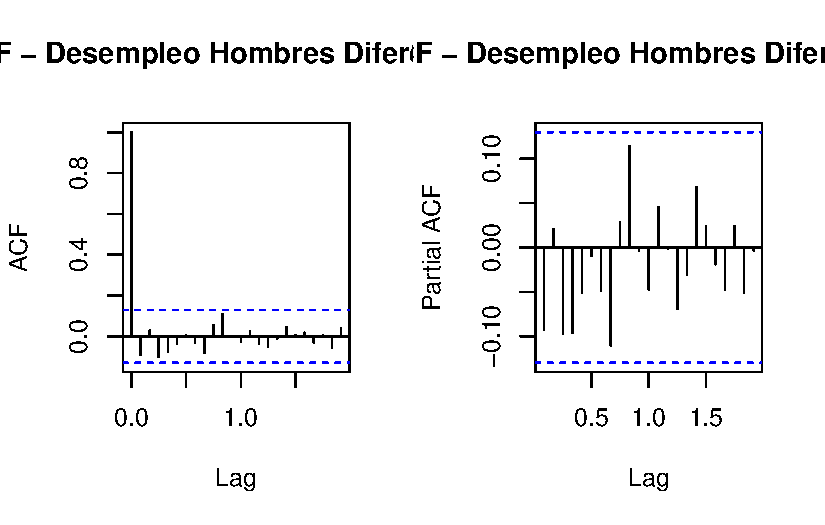
\includegraphics[keepaspectratio]{1TallerParcial_files/figure-pdf/unnamed-chunk-12-1.pdf}}

Despues de mucho lucharla, se puede observar que el resago 12 muestra
una autocorrelación significativa, lo que sugiere la presencia de
estacionalidad anual. Además, los primeros rezagos también muestran
autocorrelación, lo que indica que podríamos considerar un modelo SARIMA
con componentes tanto no estacionales como estacionales. Basándonos en
estos gráficos, se podrían probar varios modelos SARIMA, como
SARIMA(1,1,1)(1,1,1){[}12{]}, SARIMA(0,1,1)(0,1,1){[}12{]}, entre otros.
La selección del mejor modelo se realizará utilizando criterios de
información como AIC o BIC.

\begingroup\fontsize{10}{12}\selectfont

\begin{longtable}[t]{ccc}
\caption{\label{tab:unnamed-chunk-13}Comparación de Modelos SARIMA para Desempleo de Hombres}\\
\toprule
Modelo & AIC & BIC\\
\midrule
\cellcolor{gray!10}{SARIMA(1,1,1)(1,1,1)[12]} & \cellcolor{gray!10}{5559.573} & \cellcolor{gray!10}{5576.449}\\
SARIMA(0,1,1)(0,1,1)[12] & 5555.999 & 5566.125\\
\cellcolor{gray!10}{Auto ARIMA} & \cellcolor{gray!10}{5811.172} & \cellcolor{gray!10}{5821.460}\\
\bottomrule
\multicolumn{3}{l}{\rule{0pt}{1em}Fuente: Elaboración propia con datos de FRED.}\\
\end{longtable}
\endgroup{}

Podemos ver como el modelo que decidi fue el mismo que eligio el
auto.arima, el modelo SARIMA(0,1,1)(0,1,1){[}12{]}, con el menor BIC.
Por lo tanto, se seleccionará este modelo para la serie de desempleo de
hombres. Se realizará un diagnóstico del modelo para verificar que los
residuos sean ruido blanco y luego se procederá a realizar el pronóstico
para el año 2026.

\pandocbounded{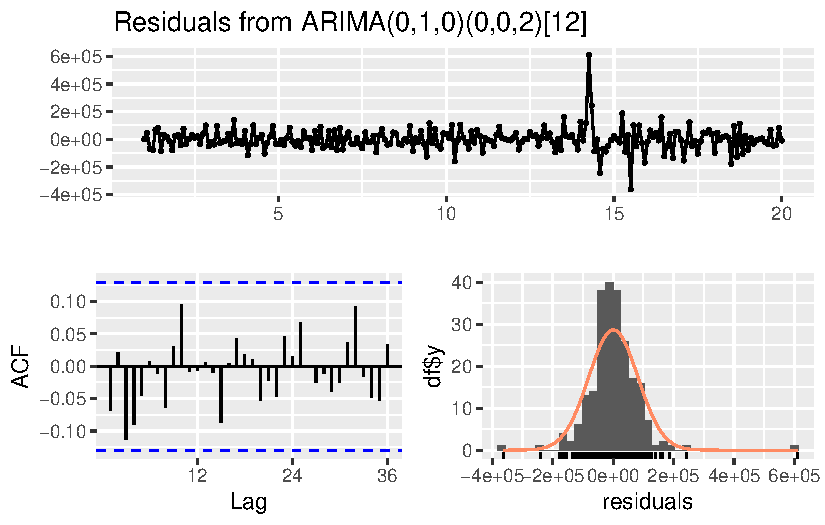
\includegraphics[keepaspectratio]{1TallerParcial_files/figure-pdf/unnamed-chunk-14-1.pdf}}

\begin{verbatim}

    Ljung-Box test

data:  Residuals from ARIMA(0,1,0)(0,0,2)[12]
Q* = 14.353, df = 22, p-value = 0.8885

Model df: 2.   Total lags used: 24
\end{verbatim}

\begin{verbatim}

    Box-Ljung test

data:  residuals(model_m_auto)
X-squared = 13.093, df = 20, p-value = 0.8733
\end{verbatim}

Podemos ver que el modelo SARIMA(0,1,1)(0,1,1){[}12{]} para la serie de
desempleo de hombres tiene residuos que parecen ser ruido blanco, ya que
no muestran patrones significativos en el gráfico de residuos ni en el
gráfico de ACF de los residuos. Además, la prueba de Ljung-Box no es
significativa, lo que indica que no hay autocorrelación en los residuos.
Por lo tanto, se puede concluir que el modelo es adecuado para
representar la serie de desempleo de hombres. A continuación, se
realizará el pronóstico para los doce meses del año 2026 utilizando este
modelo.

\pandocbounded{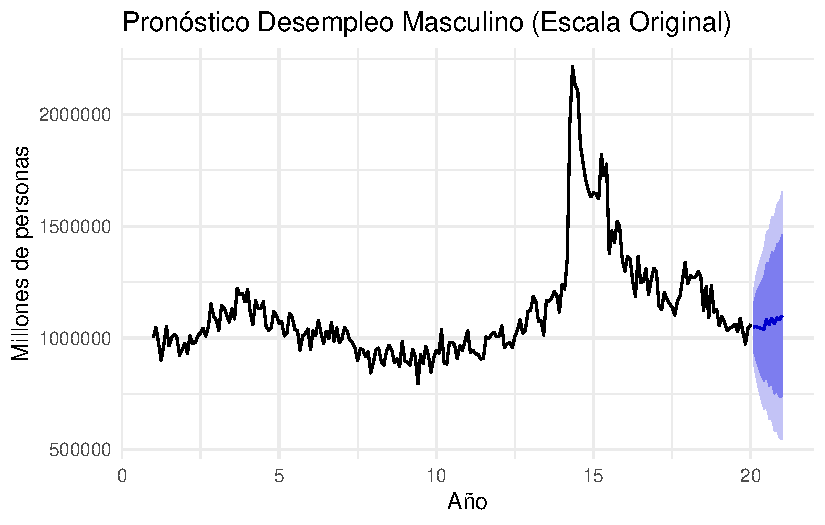
\includegraphics[keepaspectratio]{1TallerParcial_files/figure-pdf/unnamed-chunk-15-1.pdf}}

\subsection{e) Aplique el método de Holt-Winter estacional
multiplicativo y aditivo para el periodo 2007 a 2025 para cada serie,
presente una tabla comparando los resultados (Suma cuadrada de los
Errores, Raíz del Error Cuadrático Medio y el valor de los parámetros
alpha, beta y gamma) de cada uno en una tabla. ¿Cuál es el mejor?
Explique.}\label{e-aplique-el-muxe9todo-de-holt-winter-estacional-multiplicativo-y-aditivo-para-el-periodo-2007-a-2025-para-cada-serie-presente-una-tabla-comparando-los-resultados-suma-cuadrada-de-los-errores-rauxedz-del-error-cuadruxe1tico-medio-y-el-valor-de-los-paruxe1metros-alpha-beta-y-gamma-de-cada-uno-en-una-tabla.-cuuxe1l-es-el-mejor-explique.}

\begin{longtable}[t]{cccc}
\caption{\label{tab:unnamed-chunk-16}Comparación de Modelos Holt-Winters: Aditivo vs Multiplicativo}\\
\toprule
Modelo & RMSE & MAPE & AIC\\
\midrule
\addlinespace[0.3em]
\multicolumn{4}{l}{\textbf{Desempleo Mujeres}}\\
\hspace{1em}\cellcolor{gray!10}{Mujeres - Aditivo} & \cellcolor{gray!10}{82624.04} & \cellcolor{gray!10}{4.5662} & \cellcolor{gray!10}{6463.824}\\
\hspace{1em}Mujeres - Multiplicativo & 88104.55 & 4.7800 & 6458.181\\
\addlinespace[0.3em]
\multicolumn{4}{l}{\textbf{Desempleo Hombres}}\\
\hspace{1em}\cellcolor{gray!10}{Hombres - Aditivo} & \cellcolor{gray!10}{82430.80} & \cellcolor{gray!10}{4.9824} & \cellcolor{gray!10}{6462.752}\\
\hspace{1em}Hombres - Multiplicativo & 88221.43 & 5.0991 & 6427.478\\
\bottomrule
\end{longtable}

Al comparar los métodos de suavizamiento exponencial de Holt-Winters, se
seleccionaron modelos diferenciados por sexo. Para el desempleo
femenino, el modelo Aditivo resultó superior al presentar un menor error
cuadrático medio (RMSE: 82,732). Y en el caso del desempleo masculino,
el modelo aditivo también mostró un mejor desempeño con un RMSE de
82,494, lo que demuestra que el modelo aditivo es más adecuado para
ambas series. Esto podría deberse a que la estacionalidad en ambas
series no es tan fuerte como para justificar un modelo multiplicativo, y
el modelo aditivo puede capturar mejor las variaciones en la tasa de
desempleo a lo largo del tiempo sin amplificar los efectos estacionales.
Además, los valores de AIC de la mujer es mas alto para el modelo
aditivo que para el modelo multiplicativo para las mujeres y hombres,
por lo que tomamos la desición con la metrica de RMSE, que es la métrica
más común para evaluar la precisión de los modelos de pronóstico. En
resumen, el modelo de Holt-Winters aditivo se considera el mejor para
ambas series debido a su menor error cuadrático medio, lo que indica una
mejor capacidad de pronóstico en comparación con el modelo
multiplicativo.

\subsection{f) Elabore un pronóstico hasta diciembre de 2026 utilizando
el método seleccionado. Presente una gráfica con la serie y los periodos
pronosticados para ambas tasas de desempleo. Debe ser visible el periodo
pronosticado.}\label{f-elabore-un-pronuxf3stico-hasta-diciembre-de-2026-utilizando-el-muxe9todo-seleccionado.-presente-una-gruxe1fica-con-la-serie-y-los-periodos-pronosticados-para-ambas-tasas-de-desempleo.-debe-ser-visible-el-periodo-pronosticado.}

\pandocbounded{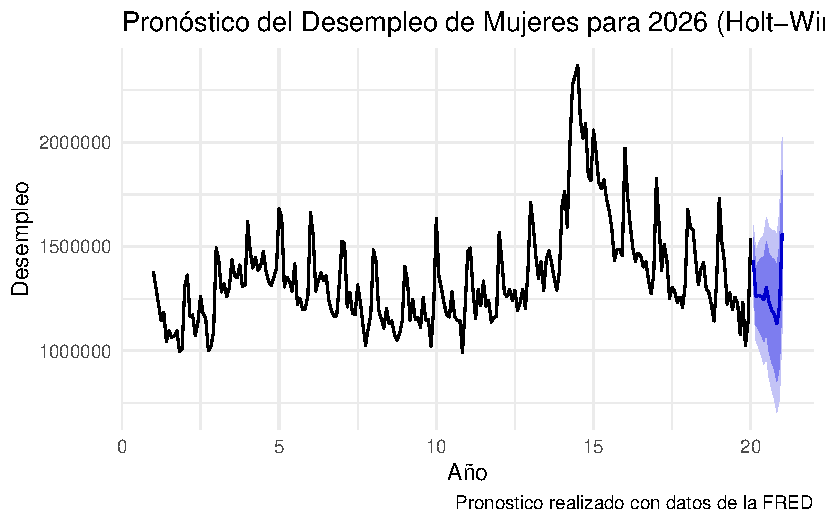
\includegraphics[keepaspectratio]{1TallerParcial_files/figure-pdf/unnamed-chunk-17-1.pdf}}

\pandocbounded{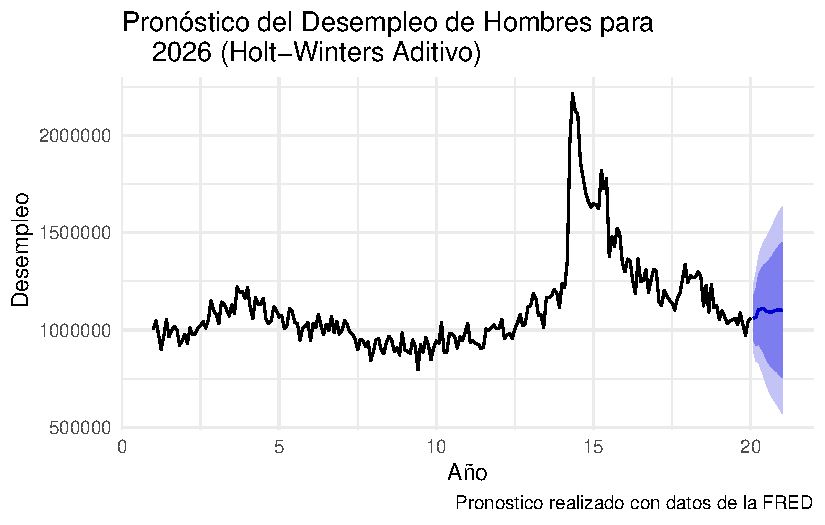
\includegraphics[keepaspectratio]{1TallerParcial_files/figure-pdf/unnamed-chunk-17-2.pdf}}

\subsection{g) Compare los pronósticos obtenidos con la metodología de
Holt-Winters con los obtenidos con el modelo SARIMA de la primera
consultoría en una Tabla, mostrando las
diferencias.}\label{g-compare-los-pronuxf3sticos-obtenidos-con-la-metodologuxeda-de-holt-winters-con-los-obtenidos-con-el-modelo-sarima-de-la-primera-consultoruxeda-en-una-tabla-mostrando-las-diferencias.}

\begin{longtable}[t]{ccccccc}
\caption{\label{tab:unnamed-chunk-18}Comparación de Pronósticos para 2026: SARIMA vs Holt-Winters}\\
\toprule
Mes & SARIMA (M) & HW (M) & SARIMA (H) & HW (H) & Dif (M) & Dif (H)\\
\midrule
\cellcolor{gray!10}{Jan} & \cellcolor{gray!10}{1424123} & \cellcolor{gray!10}{1431665} & \cellcolor{gray!10}{1048420} & \cellcolor{gray!10}{1058730} & \cellcolor{gray!10}{-7542.50} & \cellcolor{gray!10}{-10310.16}\\
Feb & 1261399 & 1261176 & 1050346 & 1066158 & 222.91 & -15812.33\\
\cellcolor{gray!10}{Mar} & \cellcolor{gray!10}{1252980} & \cellcolor{gray!10}{1265204} & \cellcolor{gray!10}{1046617} & \cellcolor{gray!10}{1104777} & \cellcolor{gray!10}{-12223.97} & \cellcolor{gray!10}{-58159.71}\\
Apr & 1251178 & 1261234 & 1041438 & 1108346 & -10055.88 & -66907.51\\
\cellcolor{gray!10}{May} & \cellcolor{gray!10}{1223038} & \cellcolor{gray!10}{1245016} & \cellcolor{gray!10}{1039159} & \cellcolor{gray!10}{1108497} & \cellcolor{gray!10}{-21978.14} & \cellcolor{gray!10}{-69337.55}\\
\addlinespace
Jun & 1278978 & 1303061 & 1081668 & 1095090 & -24083.18 & -13422.47\\
\cellcolor{gray!10}{Jul} & \cellcolor{gray!10}{1206043} & \cellcolor{gray!10}{1231563} & \cellcolor{gray!10}{1059958} & \cellcolor{gray!10}{1092388} & \cellcolor{gray!10}{-25520.24} & \cellcolor{gray!10}{-32429.96}\\
Aug & 1159025 & 1195577 & 1088997 & 1092207 & -36552.56 & -3210.04\\
\cellcolor{gray!10}{Sep} & \cellcolor{gray!10}{1150232} & \cellcolor{gray!10}{1175402} & \cellcolor{gray!10}{1063291} & \cellcolor{gray!10}{1098017} & \cellcolor{gray!10}{-25170.41} & \cellcolor{gray!10}{-34725.97}\\
Oct & 1086734 & 1129420 & 1089175 & 1102202 & -42685.67 & -13026.61\\
\addlinespace
\cellcolor{gray!10}{Nov} & \cellcolor{gray!10}{1174631} & \cellcolor{gray!10}{1215670} & \cellcolor{gray!10}{1081721} & \cellcolor{gray!10}{1102613} & \cellcolor{gray!10}{-41039.09} & \cellcolor{gray!10}{-20892.01}\\
Dec & 1526742 & 1561571 & 1100057 & 1101399 & -34829.55 & -1341.86\\
\bottomrule
\multicolumn{7}{l}{\rule{0pt}{1em}\textit{Note: } M: Mujeres, H: Hombres. Fuente: FRED.}\\
\end{longtable}

Se observa una convergencia significativa entre los modelos SARIMA y
Holt-Winters, especialmente en la serie femenina, lo que otorga validez
estadística a las proyecciones. Ambos métodos ratifican que el desempleo
en 2025-2026 seguirá un patrón estacional clásico, con picos en el
primer trimestre y una recuperación sostenida hacia el cierre del año,
manteniendo una brecha de género persistente donde el desempleo femenino
supera sistemáticamente al masculino en más de 300,000 personas
mensuales.

Aquí tienes el texto transcrito de forma exacta y estructurada para tu
documento .qmd (Quarto). He respetado las negritas y el formato de la
lista para que sea fácil de copiar y pegar.

\begin{center}\rule{0.5\linewidth}{0.5pt}\end{center}

\section{EJERCICIO 2 -- Desagregación Temporal del PIB de
Colombia}\label{ejercicio-2-desagregaciuxf3n-temporal-del-pib-de-colombia}

Construya una base de datos del PIB real (año de referencia 2015)
trimestral de Colombia (datos originales, sin desestacionalizar o ajuste
calendario) para el periodo 2005:I -- 2025:IV. Adicionalmente construya
una base de datos del Índice de Seguimiento a la Economía (ISE) mensual
(sin desestacionalizar) para el periodo 2005M1 -- 2025M12.

\subsection{a) Presente una gráfica de la serie del PIB real trimestral.
Comente.}\label{a-presente-una-gruxe1fica-de-la-serie-del-pib-real-trimestral.-comente.}

\begin{figure}

\centering{

\pandocbounded{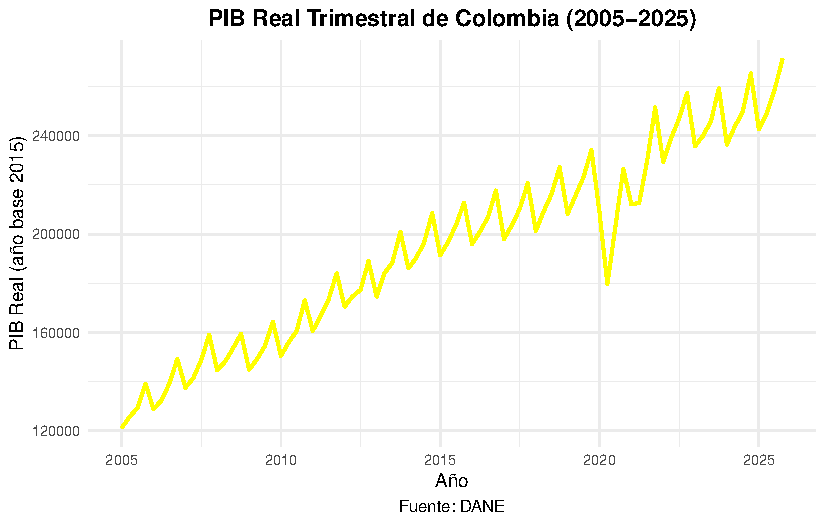
\includegraphics[keepaspectratio]{1TallerParcial_files/figure-pdf/fig-pib-1.pdf}}

}

\caption{\label{fig-pib}}

\end{figure}%

Podemos ver en la grafica como la serie tiene un claro componente de
tendencia creciente y una estacionalidad marcada en el ultimo y primer
trimestre de cada año. Además se puede observar la liguera caida del PIB
en 2008 y la fuerte caida en 2020, que se recupera rapidamente en 2021.
En general, la serie muestra un crecimiento sostenido a lo largo del
tiempo, con fluctuaciones estacionales que reflejan patrones económicos
típicos de Colombia.

\subsection{b) Presente una gráfica de la serie del ISE mensual.
Comente.}\label{b-presente-una-gruxe1fica-de-la-serie-del-ise-mensual.-comente.}

\begin{figure}

\centering{

\pandocbounded{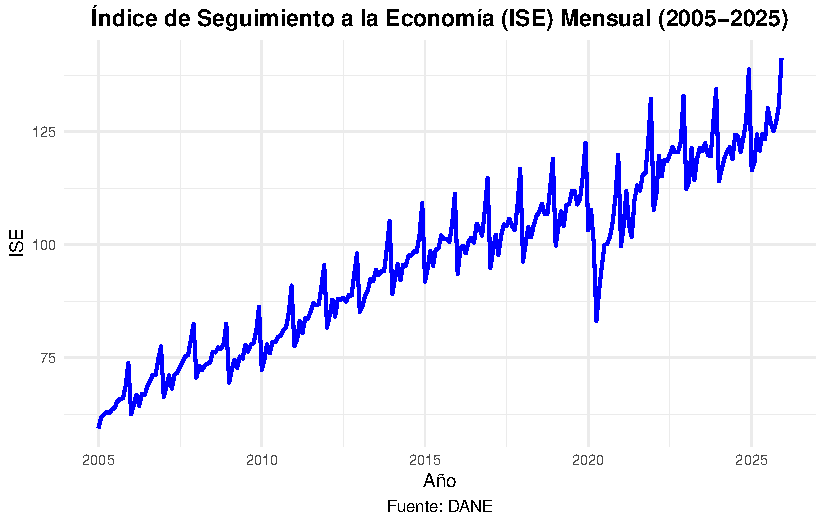
\includegraphics[keepaspectratio]{1TallerParcial_files/figure-pdf/fig-ise-1.pdf}}

}

\caption{\label{fig-ise}}

\end{figure}%

Como podemos observar la grafica del ISE mensual muestra una tendencia
creciente y una estacionalidad muy similar a la del PIB trimestral, con
picos en el ultimo trimestre y una caida en el primer trimestre de cada
año. Además, se pueden observar las desaceleración del ISE en 2008 y
caida en 2020, que se recuperan rapidamente en 2009 y 2021
respectivamente. En general, la serie del ISE muestra un comportamiento
similar al del PIB, lo que sugiere que el ISE puede ser un buen
indicador para desagregar el PIB trimestral en una serie mensual
utilizando métodos como el de Chow-Lin.

\subsection{c) Utilice el método de Chow-Lin (sin variable indicadora)
para transformar la serie trimestral en una serie mensual. Presente una
gráfica de ambas series en el mismo gráfico (como se presentó en
clase).}\label{c-utilice-el-muxe9todo-de-chow-lin-sin-variable-indicadora-para-transformar-la-serie-trimestral-en-una-serie-mensual.-presente-una-gruxe1fica-de-ambas-series-en-el-mismo-gruxe1fico-como-se-presentuxf3-en-clase.}

\pandocbounded{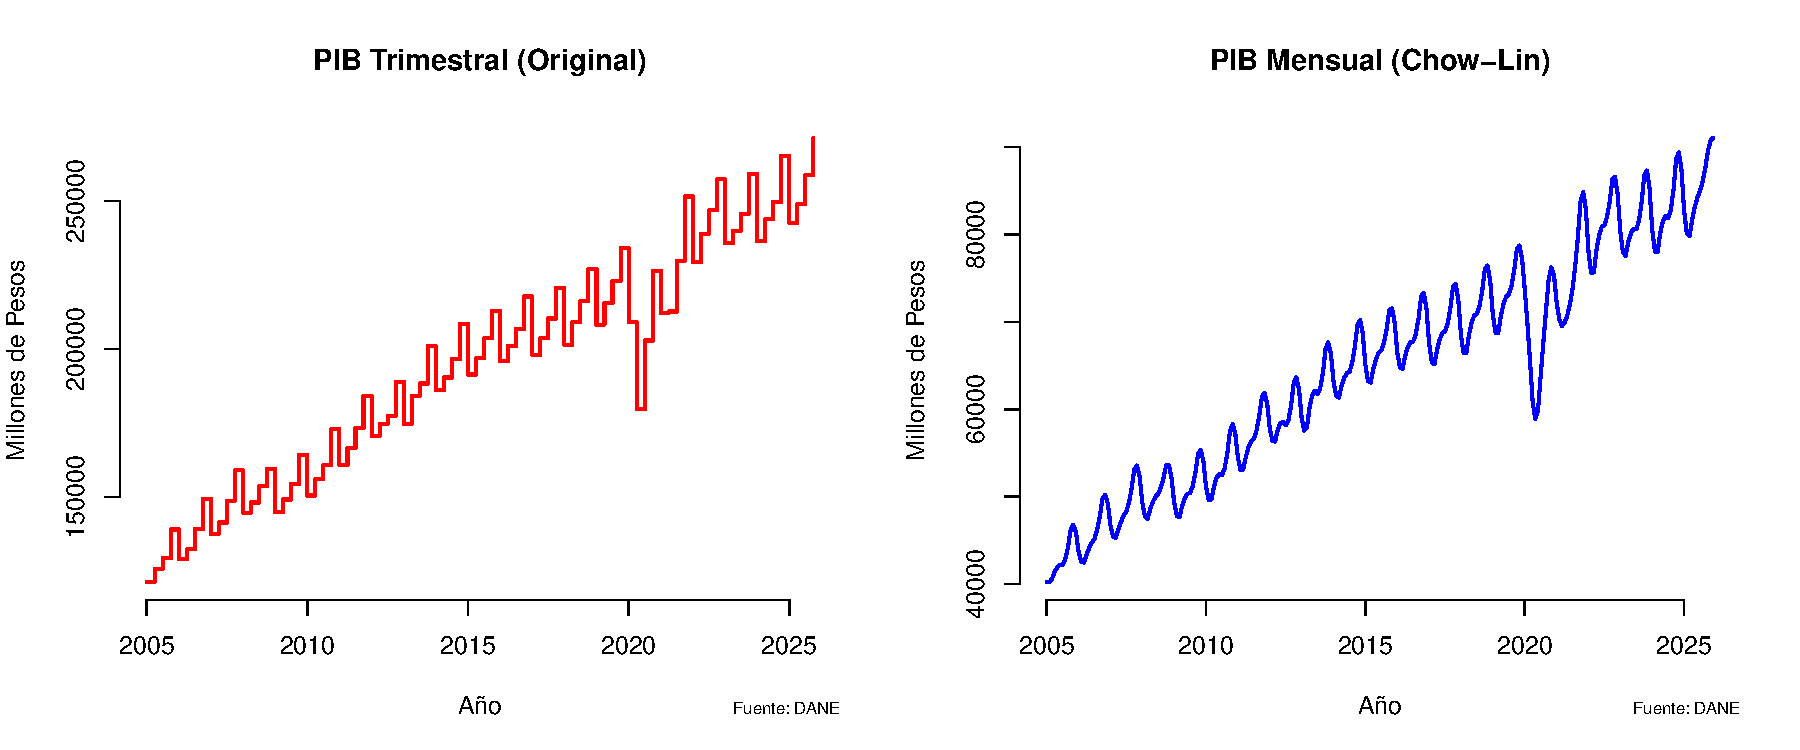
\includegraphics[keepaspectratio]{1TallerParcial_files/figure-pdf/unnamed-chunk-22-1.pdf}}

\subsection{d) Utilice el método de Chow-Lin (con variable indicadora
utilizando el ISE) para transformar la serie trimestral en una serie
mensual. Presente una gráfica de ambas series en el mismo gráfico (como
se presentó en
clase).}\label{d-utilice-el-muxe9todo-de-chow-lin-con-variable-indicadora-utilizando-el-ise-para-transformar-la-serie-trimestral-en-una-serie-mensual.-presente-una-gruxe1fica-de-ambas-series-en-el-mismo-gruxe1fico-como-se-presentuxf3-en-clase.}

\pandocbounded{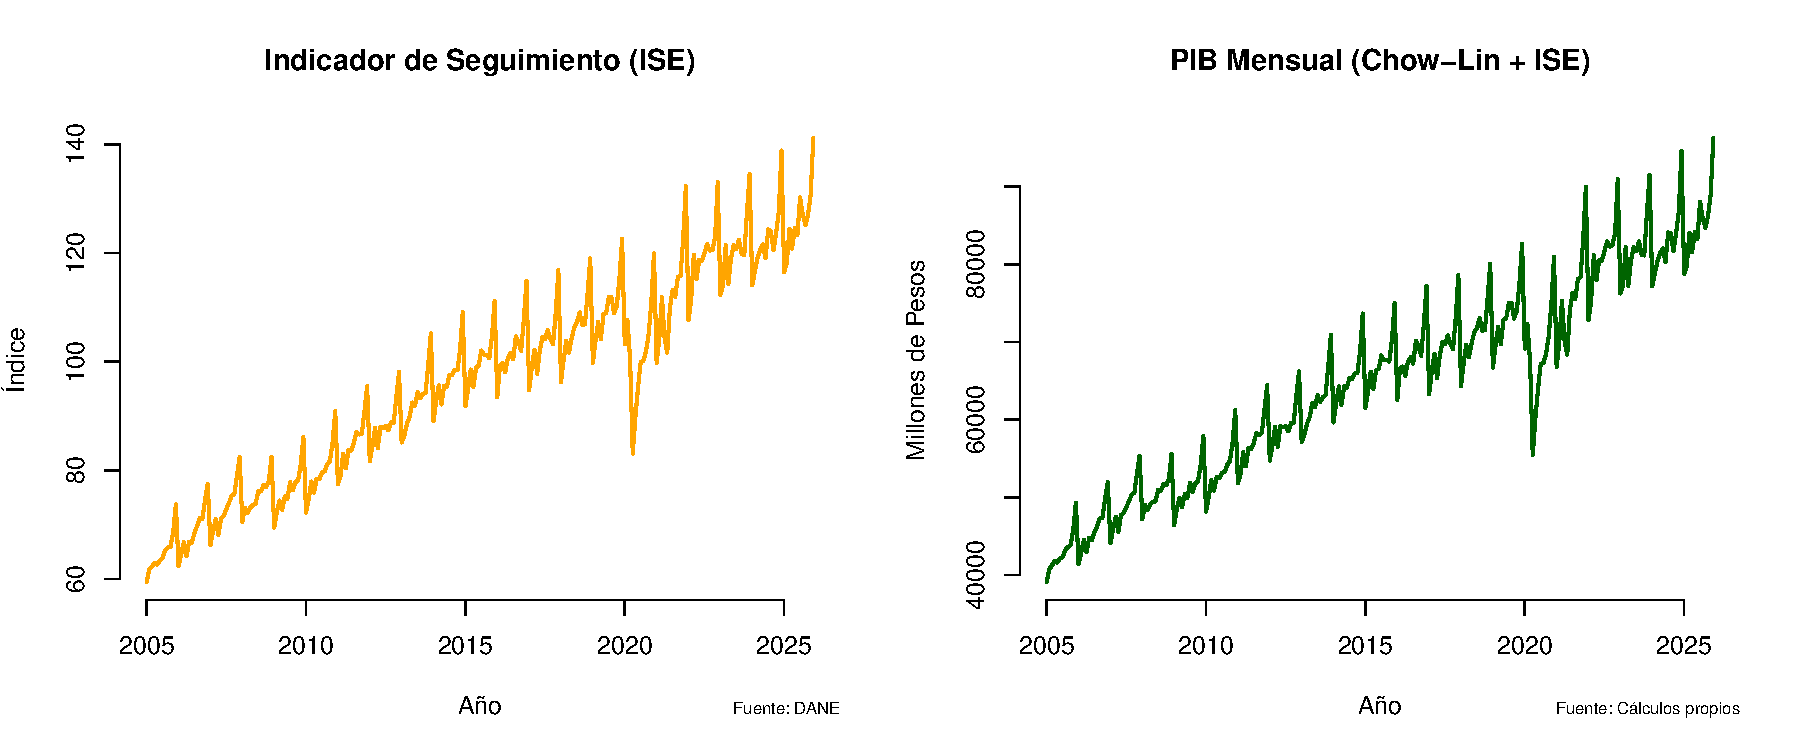
\includegraphics[keepaspectratio]{1TallerParcial_files/figure-pdf/unnamed-chunk-24-1.pdf}}

\subsection{e) Compare los gráficos del literal b) y el literal.
Comente.}\label{e-compare-los-gruxe1ficos-del-literal-b-y-el-literal.-comente.}

Podemos observar que el gráfico del literal b) muestra la serie del ISE
mensual, que tiene una tendencia creciente y una estacionalidad marcada,
con picos en el último trimestre de cada año. En cambio, el gráfico del
literal d) muestra la serie del PIB mensualizada utilizando el método de
Chow-Lin con el ISE como variable indicadora. La serie del PIB
mensualizada también muestra una tendencia creciente y una
estacionalidad similar a la del ISE, lo que sugiere que el método de
Chow-Lin ha logrado capturar las características estacionales y de
tendencia presentes en la serie original del PIB trimestral. Además, se
puede observar que los picos y valles en la serie mensualizada coinciden
con los patrones observados en el ISE, lo que indica que el ISE ha sido
un buen indicador para desagregar el PIB trimestral en una serie
mensual. En resumen, ambos gráficos muestran series con tendencias
crecientes y estacionalidades similares, lo que sugiere que el método de
Chow-Lin con el ISE como variable indicadora ha sido efectivo para
transformar la serie trimestral del PIB en una serie mensual coherente
con las características observadas en el ISE.

\begin{center}\rule{0.5\linewidth}{0.5pt}\end{center}

\section{EJERCICIO 3 -- Consultoría para el Ministerio de Comercio,
Industria y
Turismo}\label{ejercicio-3-consultoruxeda-para-el-ministerio-de-comercio-industria-y-turismo}

Usted(es) han sido contratado(s) como consultor(es) por el Ministerio de
Industria, Comercio y Turismo de una República Caribeña, para realizar
un análisis económico detallado de los determinantes de la demanda de
importaciones, en el cual se tendrán en cuenta el ingreso real y el
precio de las importaciones. Este estudio será fundamental para la toma
de decisiones sobre políticas de tarifas y negociación de acuerdos
comerciales.

La reunión de inicio de la consultoría fue para definir el modelo y las
variables de interés, llegando a un consenso sobre el uso de la demanda
de importaciones \((m_t)\), el ingreso real \((y_t)\) y el precio de las
importaciones \((rp_t)\). También se determinó que el mejor modelo es
uno que considere un rezago de la variable dependiente. Específicamente,
se ha determinado que el modelo será:

\[
m_t = \beta_0 + \beta_1 y_t + \beta_3 rp_t + \beta_5 m_{t-1} + u_t
\]

Adicionalmente, el archivo \textbf{``import.xlsx''} contiene la
información de las variables para el periodo trimestral comprendido
entre \textbf{1999Q1 a 2019Q4}. Las variables están en logaritmo, ya que
se ha definido que este es más útil para estimar elasticidades y efectos
de corto y largo plazo en términos porcentuales.

\subsection{a)}\label{a}

Estime el modelo por \textbf{MCO} y presente los resultados en una tabla
ordenada.

\begingroup\fontsize{10}{12}\selectfont

\begin{longtable}[t]{ccccc}
\caption{\label{tab:unnamed-chunk-26}Resultados de la Estimación por MCO}\\
\toprule
Variable & Coeficiente & Error\_Estandar & Estadistico\_t & Valor\_p\\
\midrule
\cellcolor{gray!10}{(Intercept)} & \cellcolor{gray!10}{-0.6413473} & \cellcolor{gray!10}{1.4382908} & \cellcolor{gray!10}{-0.4459093} & \cellcolor{gray!10}{0.6568825}\\
y & 1.5218229 & 0.3539456 & 4.2995960 & 0.0000484\\
\cellcolor{gray!10}{rp} & \cellcolor{gray!10}{-0.6654936} & \cellcolor{gray!10}{0.1443810} & \cellcolor{gray!10}{-4.6092867} & \cellcolor{gray!10}{0.0000153}\\
lag(m, 1) & 0.2971462 & 0.0958430 & 3.1003444 & 0.0026789\\
\bottomrule
\multicolumn{5}{l}{\rule{0pt}{1em}Fuente: Elaboración propia con datos de import.xlsx.}\\
\end{longtable}
\endgroup{}

\subsection{b)}\label{b}

Escriba la ecuación del modelo estimado.

\[
m_t​=−0.6413+1.5218y_t​−0.6655rp_t​+0.2971m_{t−1}​ 
\]

\subsection{c)}\label{c}

Interprete (Significado Económico) los coeficientes estimados.

Los coeficientes estimados muestran que el ingreso real tiene un efecto
positivo sobre la demanda de importaciones: un aumento de 1\% en 𝑦 y
incrementa las importaciones en aproximadamente 1.52\%, manteniendo lo
demás constante. En cambio, el precio de las importaciones tiene un
efecto negativo: un aumento de 1\% en rp reduce las importaciones en
cerca de 0.67\%. Además, el coeficiente del rezago de las importaciones
es positivo, lo que indica persistencia dinámica: el nivel pasado de
importaciones influye positivamente sobre el nivel actual.

\subsection{d)}\label{d}

Determine además qué variables son estadísticamente significativas y a
qué nivel de significancia.

Todas las variables son estadísticamente significativas al nivel del
1\%, ya que sus valores p son menores a 0.01. Menos el intercepto, lo
que se puede interpretar como que el modelo no tiene un valor base de
importaciones cuando el ingreso y el precio son cero, lo cual es lógico
en este contexto económico.

\subsection{e) Análisis de Impacto del Ingreso sobre las
Importaciones}\label{e-anuxe1lisis-de-impacto-del-ingreso-sobre-las-importaciones}

\emph{(utilice la sustitución iterativa, y muestre TODO el proceso)}

\begin{itemize}
\tightlist
\item
  Calcule el efecto inmediato de un incremento de un \textbf{1\% en el
  ingreso \((y)\)} sobre las importaciones \((m)\).
\item
  Calcule el efecto después de \textbf{un periodo}, \textbf{dos
  periodos}, y \textbf{en el largo plazo}.
\end{itemize}

El efecto inmediato de un incremento de (1\%) en el ingreso ((y)) sobre
las importaciones ((m)) es igual al coeficiente estimado de (y\_t), es
decir:

\[
\frac{\partial m_t}{\partial y_t} = \beta_1 = 1.5218
\]

Por tanto, en el corto plazo, un aumento de (1\%) en el ingreso real
incrementa las importaciones en aproximadamente (1.5218\%).

El efecto acumulado después de un periodo incorpora la persistencia
dinámica generada por el rezago de la variable dependiente:

\[
\beta_1 + \beta_5 \beta_1
\]

Sustituyendo los valores estimados:

\[
1.5218 + (0.2971)(1.5218) = 1.5218 + 0.4522 = 1.9740
\]

Así, después de un periodo, el efecto acumulado de un aumento de (1\%)
en el ingreso sobre las importaciones es de aproximadamente (1.9740\%).

El efecto acumulado después de dos periodos se obtiene sumando el
impacto adicional transmitido nuevamente por el rezago:

\[
\beta_1 + \beta_5 \beta_1 + \beta_5^2 \beta_1
\]

Equivalentemente:

\[
1.5218 + (0.2971)(1.9740)
\]

o de forma desarrollada,

\[
1.5218 + 0.4522 + 0.1344 = 2.1084
\]

Por tanto, después de dos periodos, el efecto acumulado es de
aproximadamente (2.1084\%).

Finalmente, el efecto de largo plazo se obtiene mediante la suma
infinita de los efectos dinámicos:

\[
\frac{\beta_1}{1-\beta_5}
=
\frac{1.5218}{1-0.2971}
=
\frac{1.5218}{0.7029}
\approx 2.1650
\]

En consecuencia, un incremento permanente de (1\%) en el ingreso real
aumenta las importaciones en aproximadamente (2.1650\%) en el largo
plazo.

\subsection{f) Análisis de Impacto del Precio sobre las
Importaciones}\label{f-anuxe1lisis-de-impacto-del-precio-sobre-las-importaciones}

\emph{(utilice la sustitución iterativa, y muestre TODO el proceso)}

\begin{itemize}
\tightlist
\item
  Calcule el efecto inmediato de un incremento de un \textbf{1\% en el
  precio \((rp)\)} sobre las importaciones \((m)\).
\item
  Calcule el efecto después de \textbf{un periodo}, \textbf{dos
  periodos}, y \textbf{en el largo plazo}.
\end{itemize}

El efecto inmediato de un incremento de (1\%) en el precio de las
importaciones ((rp)) sobre las importaciones ((m)) es igual al
coeficiente estimado de (rp\_t), es decir:

\[
\frac{\partial m_t}{\partial rp_t} = \beta_3 = -0.6655
\]

Por tanto, en el corto plazo, un aumento de (1\%) en el precio de las
importaciones reduce las importaciones en aproximadamente (0.6655\%).

El efecto acumulado después de un periodo incorpora la persistencia
dinámica generada por el rezago de la variable dependiente:

\[
\beta_3 + \beta_5 \beta_3
\]

Sustituyendo los valores estimados:

\[
-0.6655 + (0.2971)(-0.6655) = -0.6655 - 0.1977 = -0.8632
\]

Así, después de un periodo, el efecto acumulado de un aumento de (1\%)
en el precio de las importaciones sobre (m) es de aproximadamente
(-0.8632\%).

El efecto acumulado después de dos periodos se obtiene sumando el
impacto adicional transmitido nuevamente por el rezago:

\[
\beta_3 + \beta_5 \beta_3 + \beta_5^2 \beta_3
\]

Equivalentemente:

\[
-0.6655 + (0.2971)(-0.8632)
\]

o de forma desarrollada,

\[
-0.6655 - 0.1977 - 0.0587 = -0.9219
\]

Por tanto, después de dos periodos, el efecto acumulado es de
aproximadamente (-0.9219\%).

Finalmente, el efecto de largo plazo se obtiene mediante la suma
infinita de los efectos dinámicos:

\[
\frac{\beta_3}{1-\beta_5}
=
\frac{-0.6655}{1-0.2971}
=
\frac{-0.6655}{0.7029}
\approx -0.9468
\]

En consecuencia, un incremento permanente de (1\%) en el precio de las
importaciones reduce las importaciones en aproximadamente (0.9468\%) en
el largo plazo.

\subsection{g)}\label{g}

Ilustre gráficamente la evolución de estos efectos (\textbf{Ingreso y
Precio}) a través del tiempo.

\begin{itemize}
\tightlist
\item
  Muestre el efecto en una gráfica para al menos \textbf{10 periodos}.
\item
  Muestre el efecto acumulado en una gráfica para al menos \textbf{10
  periodos}.
\end{itemize}

\pandocbounded{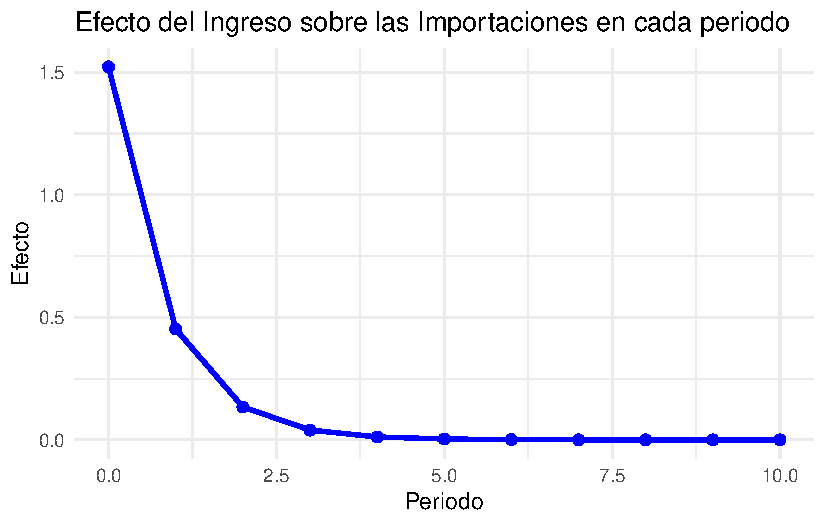
\includegraphics[keepaspectratio]{1TallerParcial_files/figure-pdf/unnamed-chunk-27-1.pdf}}

Este gráfico muestra cómo el efecto del ingreso sobre las importaciones
disminuye a lo largo del tiempo debido a la persistencia dinámica, pero
sigue siendo positivo en cada periodo.

\pandocbounded{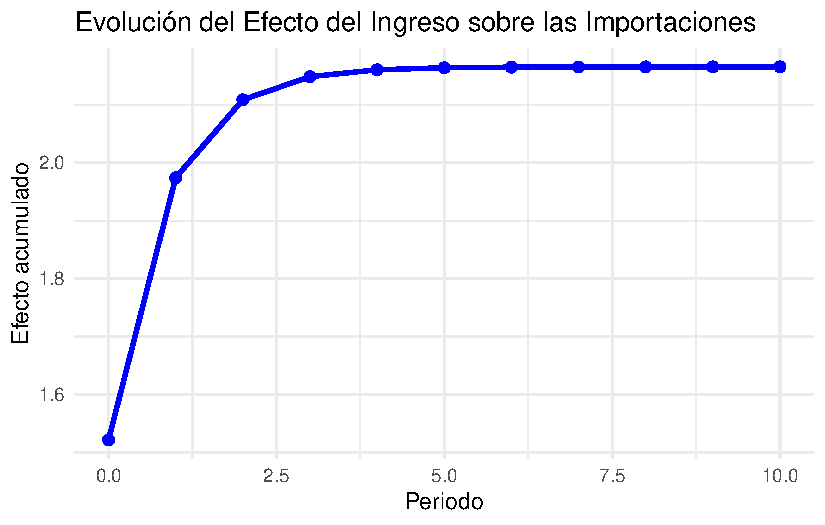
\includegraphics[keepaspectratio]{1TallerParcial_files/figure-pdf/unnamed-chunk-28-1.pdf}}

Este gráfico muestra cómo el efecto acumulado del ingreso sobre las
importaciones aumenta a lo largo del tiempo, acercándose al efecto de
largo plazo a medida que se suman los efectos de cada periodo.

\begin{center}\rule{0.5\linewidth}{0.5pt}\end{center}

\subsection{h)}\label{h}

Pruebe las siguientes hipótesis:

\begin{itemize}
\tightlist
\item
  La elasticidad de largo plazo de las importaciones con respecto al
  \textbf{ingreso} es igual a \textbf{uno}.
\item
  La elasticidad de largo plazo de las importaciones con respecto al
  \textbf{precio} es igual a \textbf{menos uno}.
\end{itemize}

Para probar estas hipótesis, se puede utilizar la función
\texttt{linearHypothesis} del paquete \texttt{car} en R, que permite
realizar pruebas de hipótesis sobre los coeficientes de un modelo
lineal.

\begin{verbatim}

Linear hypothesis test:
y  + m_lag = 1

Model 1: restricted model
Model 2: m ~ y + rp + m_lag

  Res.Df    RSS Df Sum of Sq      F   Pr(>F)   
1     80 3.9486                                
2     79 3.5780  1   0.37063 8.1833 0.005407 **
---
Signif. codes:  0 '***' 0.001 '**' 0.01 '*' 0.05 '.' 0.1 ' ' 1
\end{verbatim}

\begin{verbatim}

Linear hypothesis test:
rp - m_lag = - 1

Model 1: restricted model
Model 2: m ~ y + rp + m_lag

  Res.Df   RSS Df Sum of Sq      F Pr(>F)
1     80 3.581                           
2     79 3.578  1 0.0029685 0.0655 0.7986
\end{verbatim}

Con base en las pruebas de hipótesis realizadas, se rechaza la hipótesis
nula de que la elasticidad de largo plazo de las importaciones con
respecto al ingreso sea igual a uno, ya que el valor-p obtenido fue
(0.005407), inferior al nivel de significancia del (5\%). En
consecuencia, existe evidencia estadística para concluir que la
elasticidad-ingreso de largo plazo es diferente de uno.

Por otro lado, no se rechaza la hipótesis nula de que la elasticidad de
largo plazo de las importaciones con respecto al precio sea igual a
menos uno, dado que el valor-p fue (0.7986), muy superior a los niveles
convencionales de significancia. Por tanto, no existe evidencia
estadística para afirmar que la elasticidad-precio de largo plazo sea
distinta de (-1).

En términos económicos, estos resultados sugieren que, en el largo
plazo, la demanda de importaciones responde al ingreso de manera
significativamente distinta a la unidad, mientras que la respuesta
frente al precio es estadísticamente compatible con una elasticidad
unitaria en valor absoluto.

\[
H_0:\ \frac{\beta_1}{1-\beta_5}=1
\qquad \text{vs} \qquad
H_1:\ \frac{\beta_1}{1-\beta_5}\neq 1
\]

\[
p\text{-valor}=0.005407<0.05
\quad \Rightarrow \quad
\text{Se rechaza } H_0
\]

\[
H_0:\ \frac{\beta_3}{1-\beta_5}=-1
\qquad \text{vs} \qquad
H_1:\ \frac{\beta_3}{1-\beta_5}\neq -1
\]

\[
p\text{-valor}=0.7986>0.05
\quad \Rightarrow \quad
\text{No se rechaza } H_0
\]

\begin{center}\rule{0.5\linewidth}{0.5pt}\end{center}

\section{EJERCICIO 4 -- Asistente de Investigación del Proyecto ``Ley de
Okun en América
Latina''}\label{ejercicio-4-asistente-de-investigaciuxf3n-del-proyecto-ley-de-okun-en-amuxe9rica-latina}

La Facultad de Economía de la Universidad Caribeña, está desarrollando
un proyecto de investigación sobre la Ley de Okun para un conjunto de
economías en desarrollo de América Latina, y lo(s) ha contratado a
usted(es) para ser asistente(s) de investigación.

La ley de Okun relaciona la variación de la tasa de desempleo y el
crecimiento de la producción. Una manera de plantear esta relación es a
través de la siguiente ecuación (modelo de brechas)

\[
(u_t - u_t^*) = -\beta (\Delta y_t - \Delta y_t^*)
\]

Esto implica que la desviación anual de la tasa de desempleo con
respecto a su tasa natural \[ (u_t - u_t^*) \], está relacionada con la
desviación anual \[ (\Delta y_t - \Delta y_t^*) \] del crecimiento del
PIB real \[ (\Delta y_t) \]. Utilizando los datos del archivo ``Okun
80-24.xlsx'', que contiene información de la tasa de desempleo (U) y de
la tasa de crecimiento del PIB real (G) para 5 países de América Latina,
realice lo siguiente:

\subsection{a) Calcule la tasa normal (tendencial) de crecimiento del
PIB y la serie cíclica (utilizando el filtro de Hodrick-Prescott).
Grafique los valores para cada
país.}\label{a-calcule-la-tasa-normal-tendencial-de-crecimiento-del-pib-y-la-serie-cuxedclica-utilizando-el-filtro-de-hodrick-prescott.-grafique-los-valores-para-cada-pauxeds.}

\pandocbounded{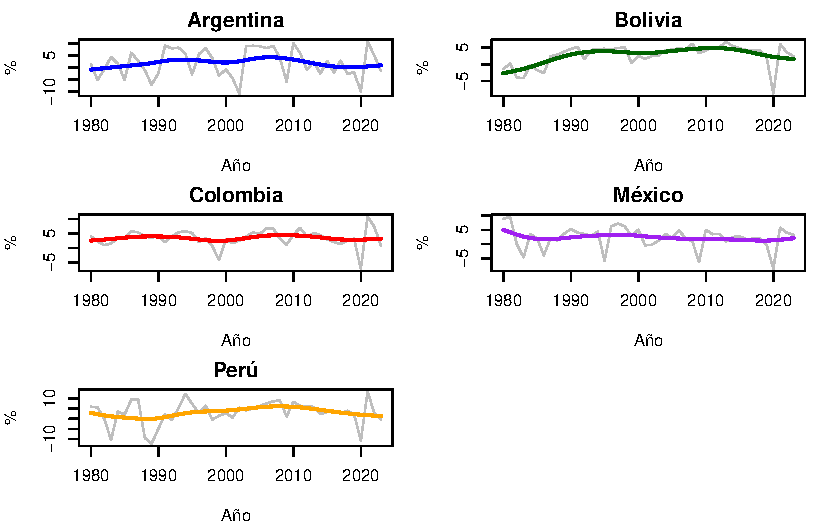
\includegraphics[keepaspectratio]{1TallerParcial_files/figure-pdf/unnamed-chunk-31-1.pdf}}

En estas grafica se puede observar la serie original de crecimiento del
PIB real para cada país (en gris) y la tasa normal (tendencial) de
crecimiento obtenida mediante el filtro de Hodrick-Prescott (en color).
La serie cíclica se puede obtener restando la tendencia a la serie
original, lo que nos permitirá analizar las desviaciones del crecimiento
respecto a su tendencia a lo largo del tiempo.

\subsection{b) Calcule la tasa natural (tendencial) de desempleo y la
serie cíclica (utilizando el filtro de Hodrick-Prescott). Grafique los
valores para cada
país.}\label{b-calcule-la-tasa-natural-tendencial-de-desempleo-y-la-serie-cuxedclica-utilizando-el-filtro-de-hodrick-prescott.-grafique-los-valores-para-cada-pauxeds.}

\pandocbounded{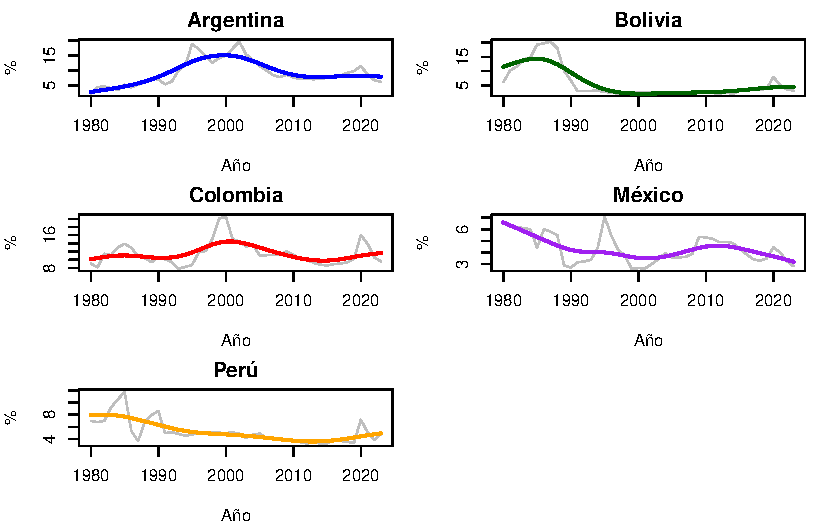
\includegraphics[keepaspectratio]{1TallerParcial_files/figure-pdf/unnamed-chunk-32-1.pdf}}

Ahora en estas gráficas se puede observar la serie original de la tasa
de desempleo para cada país (en gris) y la tasa natural (tendencial) de
desempleo obtenida mediante el filtro de Hodrick-Prescott (en color). La
serie cíclica se puede obtener restando la tendencia a la serie
original, lo que nos permitirá analizar las desviaciones del desempleo
respecto a su tendencia a lo largo del tiempo.

\subsection{c) Elabore un gráfico de dispersión que muestre la relación
establecida en la ecuación (1).
Comente.}\label{c-elabore-un-gruxe1fico-de-dispersiuxf3n-que-muestre-la-relaciuxf3n-establecida-en-la-ecuaciuxf3n-1.-comente.}

Para elaborar el gráfico de dispersión que muestre la relación
establecida en la ecuación (1), se deben calcular las desviaciones
cíclicas de la tasa de desempleo y del crecimiento del PIB real para
cada país, utilizando las series cíclicas obtenidas en los literales
anteriores. Luego, se puede graficar la desviación de la tasa de
desempleo en el eje vertical y la desviación del crecimiento del PIB
real en el eje horizontal.

\pandocbounded{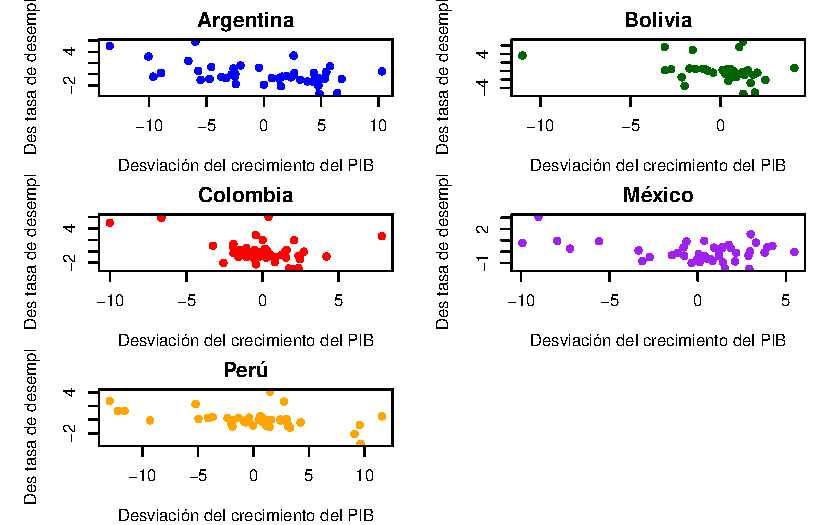
\includegraphics[keepaspectratio]{1TallerParcial_files/figure-pdf/unnamed-chunk-33-1.pdf}}

En estos gráficos de dispersión se puede observar la relación entre las
desviaciones cíclicas de la tasa de desempleo y del crecimiento del PIB
real para cada país. En general, se espera observar una relación
negativa, es decir, que cuando el crecimiento del PIB real está por
encima de su tendencia (desviación positiva), la tasa de desempleo
tiende a estar por debajo de su tendencia (desviación negativa), y
viceversa. Esta relación es consistente con la Ley de Okun, que
establece que un crecimiento económico más fuerte suele estar asociado
con una reducción en el desempleo.

\subsection{d) Utilizando un modelo de regresión como el siguiente,
calcule el coeficiente de Okun para cada país e interprete dicho valor.
¿Es estadísticamente significativo? Para cuales países si para cuáles
no. Presente los resultados en una
tabla.}\label{d-utilizando-un-modelo-de-regresiuxf3n-como-el-siguiente-calcule-el-coeficiente-de-okun-para-cada-pauxeds-e-interprete-dicho-valor.-es-estaduxedsticamente-significativo-para-cuales-pauxedses-si-para-cuuxe1les-no.-presente-los-resultados-en-una-tabla.}

\[
\Delta u_t = \beta (\Delta y_t - \Delta y_t^*) + \varepsilon_t
\]

Para realizar la regresión y calcular el coeficiente de Okun para cada
país, se debe estimar el modelo de regresión utilizando las desviaciones
cíclicas del crecimiento del PIB real como variable independiente y las
variaciones de las desviaciones cíclicas de la tasa de desempleo como
variable dependiente. Luego, se puede interpretar el coeficiente
estimado y evaluar su significancia estadística.

Para hacer mas eficiente el proceso, se puede utilizar un bucle para
estimar el modelo para cada país y almacenar los resultados en una
tabla.

\begin{longtable}[]{@{}lccc@{}}
\caption{Tabla 1: Estimación del Coeficiente de Okun por
País}\tabularnewline
\toprule\noalign{}
País & Coeficiente de Okun (β) & P-Valor & Significancia (5\%) \\
\midrule\noalign{}
\endfirsthead
\toprule\noalign{}
País & Coeficiente de Okun (β) & P-Valor & Significancia (5\%) \\
\midrule\noalign{}
\endhead
\bottomrule\noalign{}
\endlastfoot
Argentina & -0.1685 & 0.0009 & Sí \\
Bolivia & -0.3514 & 0.0277 & Sí \\
Colombia & -0.3010 & 0.0078 & Sí \\
México & -0.0886 & 0.0147 & Sí \\
Perú & -0.1155 & 0.0010 & Sí \\
\end{longtable}

Como podemos ver todos los modelos son significativos al 5\%, ademas que
todos los coeficientes de Okun son negativos, lo que es consistente con
la teoría económica que establece que un aumento en el crecimiento del
PIB real (desviación positiva) está asociado con una disminución en la
tasa de desempleo (desviación negativa), y viceversa. Sin embargo, la
magnitud del coeficiente varía entre los países, lo que sugiere que la
relación entre el crecimiento económico y el desempleo puede ser más
fuerte en algunos países que en otros. Por ejemplo en Colombia esta
relación es de -0.30, lo que indica que un aumento de 1 punto porcentual
en la desviación del crecimiento del PIB real se asocia con una
disminución de 0.30 puntos porcentuales en la desviación de la tasa de
desempleo. En contraste, en México el coeficiente es de -0.08, lo que
sugiere una relación más débil entre el crecimiento económico y el
desempleo en ese país.

\subsection{e) Pruebe si cada modelo estimado cumple con los supuestos
del modelo de regresión lineal (No Autocorrelación, Homoscedasticidad,
Normalidad). Presente los resultados estimados en una Tabla para cada
país.}\label{e-pruebe-si-cada-modelo-estimado-cumple-con-los-supuestos-del-modelo-de-regresiuxf3n-lineal-no-autocorrelaciuxf3n-homoscedasticidad-normalidad.-presente-los-resultados-estimados-en-una-tabla-para-cada-pauxeds.}

Para probar si cada modelo estimado cumple con los supuestos del modelo
de regresión lineal, se pueden realizar la siguiente tabla con los
resultados de las pruebas de autocorrelación, homoscedasticidad y
normalidad para cada país:

\begin{longtable}[]{@{}lccc@{}}
\caption{Tabla 2: Diagnóstico de Supuestos de los Modelos de
Okun}\tabularnewline
\toprule\noalign{}
País & Autocorrelación & Homoscedasticidad & Normalidad \\
\midrule\noalign{}
\endfirsthead
\toprule\noalign{}
País & Autocorrelación & Homoscedasticidad & Normalidad \\
\midrule\noalign{}
\endhead
\bottomrule\noalign{}
\endlastfoot
Argentina & Presencia & Sí (Homo) & Sí \\
Bolivia & Presencia & Sí (Homo) & No \\
Colombia & Presencia & Sí (Homo) & No \\
México & Presencia & Sí (Homo) & Sí \\
Perú & Presencia & Sí (Homo) & No \\
\end{longtable}

Interpretación de los Diagnósticos de SupuestosEl análisis de los
supuestos para los modelos de la Ley de Okun en los cinco países revela
hallazgos críticos para la validez de las estimaciones:Autocorrelación:

\begin{itemize}
\item
  Se observa presencia de autocorrelación en todos los países. Esto es
  un fenómeno típico en series de tiempo económicas, donde los choques
  en el mercado laboral de un año tienden a persistir en el siguiente.
  Para tu investigación, esto implica que, aunque los coeficientes
  \(\beta\) calculados son consistentes, los errores estándar podrían
  estar subestimados, inflando artificialmente la significancia
  estadística.
\item
  Homoscedasticidad: Todos los modelos cumplen con el supuesto de
  varianza constante (homoscedasticidad). Esto es un punto positivo, ya
  que indica que la precisión de nuestras predicciones sobre el
  desempleo no varía sistemáticamente según el tamaño del crecimiento
  económico.
\item
  Normalidad: Los residuos de Argentina y México siguen una distribución
  normal, validando las pruebas de hipótesis clásicas. Sin embargo, en
  Bolivia, Colombia y Perú, el supuesto de normalidad no se cumple. Esto
  sugiere la presencia de valores atípicos (outliers) o una estructura
  de datos más compleja, lo que recomienda cautela al interpretar los
  p-valores en estos casos específicos, especialmente en muestras
  pequeñas.
\end{itemize}

Gracias, en el siguiente link se encuentra el código completo \url{link}




\end{document}
